\section{Welcome to the Open Physics Education
Network}\label{welcome-to-the-open-physics-education-network}

\begin{figure}
\centering
\pandocbounded{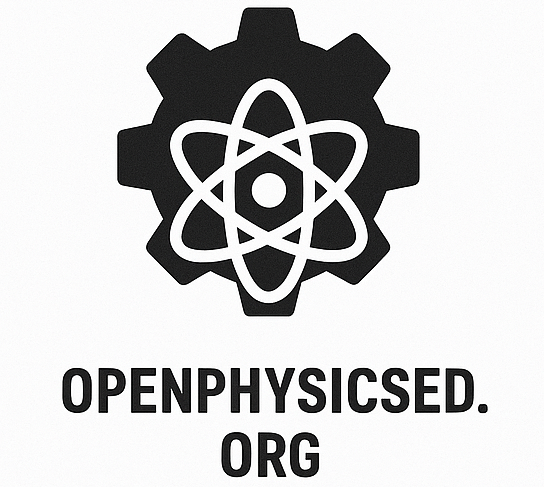
\includegraphics[keepaspectratio,alt={Open Physics Education Network Logo}]{./images/logo.png}}
\caption{Open Physics Education Network Logo}
\end{figure}

\href{https://open-physics-ed-org.github.io/}{openphysicsed.org} is a
collaborative, open-source project dedicated to building accessible,
high-quality, and modern educational resources for physics and
computational science. Our mission is to lower barriers to learning by
providing free, open, and adaptable materials for students, educators,
and lifelong learners everywhere.

\subsection{What We Offer}\label{what-we-offer}

\begin{itemize}
\tightlist
\item
  \textbf{Accessible, open resources} for physics and computational
  science
\item
  \textbf{Modern, semantic, and screen-reader-friendly design}
\item
  \textbf{Collaborative development}---anyone can contribute
\item
  \textbf{Free to use, modify, and distribute}
\item
  \textbf{Open-source tools, materials, and a wide variety of formats}
\end{itemize}

\subsection{Courses and Materials}\label{courses-and-materials}

We are actively transcribing and deploying resources for:

\begin{itemize}
\tightlist
\item
  \textbf{Introductory Mechanics}
\item
  \textbf{Introductory Electromagnetism}
\item
  \textbf{Sophomore-level Classical Mechanics} (see
  \href{https://open-physics-ed-org.github.io/modern-classical-mechanics/}{Modern
  Classical Mechanics})
\item
  \textbf{Junior-level Electromagnetism}
\item
  \textbf{Mathematical Methods}
\end{itemize}

In the future, we plan to expand to:

\begin{itemize}
\tightlist
\item
  \textbf{Modern Physics}
\item
  \textbf{Quantum Physics}
\item
  \textbf{Statistical Mechanics}
\item
  \textbf{Community Proposed Areas}
\end{itemize}

\subsection{Our Philosophy}\label{our-philosophy}

The Open Physics Education Network is guided by the following
principles: 1. \textbf{Openness:} All materials are open source and free
to use, modify, and distribute under non-commercial licenses. 2.
\textbf{Accessibility:} We strive to meet and exceed accessibility
standards, ensuring our resources are usable by everyone. 3.
\textbf{Collaboration:} We welcome contributions from students,
educators, developers, and the broader community. 4.
\textbf{Simplicity:} Our sites and materials are intentionally simple
and easy to use, modify, and distribute.

\subsection{Get Involved}\label{get-involved}

We welcome your feedback, suggestions, and contributions!

Visit our
\href{https://github.com/open-physics-ed/open-physics-ed-org.github.io}{GitHub
repository} to get started, or reach out to
\href{https://dannycab.github.io/}{Danny Caballero} for more
information.

The easiest way to help is to
\href{https://github.com/open-physics-ed-org/open-physics-ed-org.github.io/issues}{report
an issue} or if you are so kind to clean some code,
\href{https://github.com/open-physics-ed-org/open-physics-ed-org.github.io/pulls}{issue
a pull request}.

\href{https://github.com/open-physics-ed-org/open-physics-ed-org.github.io}{\pandocbounded{\includegraphics[keepaspectratio,alt={GitHub Repo stars}]{https://img.shields.io/github/stars/open-physics-ed-org/open-physics-ed-org.github.io?style=social}}}
\href{https://github.com/open-physics-ed-org/open-physics-ed-org.github.io/issues}{\pandocbounded{\includegraphics[keepaspectratio,alt={GitHub issues}]{https://img.shields.io/github/issues/open-physics-ed-org/open-physics-ed-org.github.io}}}
\href{https://github.com/open-physics-ed-org/open-physics-ed-org.github.io/pulls}{\pandocbounded{\includegraphics[keepaspectratio,alt={GitHub pull requests}]{https://img.shields.io/github/issues-pr/open-physics-ed-org/open-physics-ed-org.github.io}}}

\subsection{License}\label{license}

The site including written content and the build process are licensed
with the
\href{https://creativecommons.org/licenses/by-nc-sa/4.0/}{Creative
Commons Attribution-NonCommercial-ShareAlike 4.0 International License}.

\href{https://github.com/open-physics-ed-org/open-physics-ed-org.github.io/blob/main/LICENSE}{\pandocbounded{\includegraphics[keepaspectratio,alt={GitHub license}]{https://img.shields.io/github/license/open-physics-ed-org/open-physics-ed-org.github.io}}}

\subsection{Releases}\label{releases}

Releases for this repo are limited to changes to \texttt{build.py} the
code that builds the site from markdown. The build system is simpler and
less feature rich than other static site generators, but can be used to
stand up a similarly simple site.

\href{https://github.com/open-physics-ed-org/open-physics-ed-org.github.io/releases}{\pandocbounded{\includegraphics[keepaspectratio,alt={Releases}]{https://img.shields.io/github/v/release/open-physics-ed-org/open-physics-ed-org.github.io?include_prereleases}}}
